\documentclass[a4paper,dvipdfmx]{jarticle}
\usepackage{amsmath}
\usepackage{bm}
\usepackage{physics}
\usepackage{pdfpages}
\usepackage{here}
\usepackage{titlesec}
\titleformat*{\section}{\large\bfseries}
\titleformat*{\subsection}{\normalsize\bfseries}

\renewcommand{\thesection}{問題\arabic{section}}
\renewcommand{\thesubsection}{(\arabic{subsection})}


\begin{document}

\title{シミュレーション実習 期末レポート}
\author{262201018 在田 陽一}
\date{2022/07/03}
\maketitle


% 問題1
\section{}

% (1)
\subsection{}

\noindent
与えられたLangevin方程式を無次元化する.
条件より$\bm{F}_B(t)=\sqrt{\frac{2k_BT\zeta}{\Delta t}}\bm{R}_G$. 
また $v=\frac{a}{t_0}\tilde{v}$, $t=t_0\tilde{t}$ より

\begin{align*}
    \frac{d\bm{v}}{dt} &= \frac{a}{t_0}\frac{d\bm{\tilde{v}}}{d\tilde{t}} \frac{d\tilde{t}}{dt} \\ 
    &= \frac{a}{t_0^2} \frac{d\bm{\tilde{v}}}{d\tilde{t}}  \tag{1.1}
\end{align*}

\noindent
であるので, それぞれ代入すると

\begin{equation}
    m \frac{a}{t_0^2} \bm{\dot{\tilde{v}}} = -\zeta \frac{a}{t_0} \bm{\tilde{v}} 
    + \sqrt{\frac{2k_BT \zeta}{t_0 \Delta \tilde{t}}}\bm{R}_G \tag{1.2}
\end{equation}

\noindent
式(1.2)に $t_D=\frac{m}{\zeta}$, $t_B=\frac{a^2 \zeta}{k_BT}$ を代入すると

\begin{equation}
    \frac{a\zeta t_D}{t_0^2} \bm{\dot{\tilde{v}}} = -\frac{a\zeta}{t_0} \bm{\tilde{v}} 
    + \sqrt{\frac{2a^2\zeta ^2}{t_Bt_0 \Delta \tilde{t}}}\bm{R}_G \tag{1.3} 
\end{equation}
両辺に $\frac{t_0}{\zeta a}$ をかけると

\begin{equation}
    \frac{t_D}{t_0} \bm{\dot{\tilde{v}}} = -\bm{\tilde{v}} 
    + \sqrt{\frac{2t_0}{t_B\Delta \tilde{t}}}\bm{R}_G \tag{1.4} 
\end{equation}
となり, 題意に適する.


% (2)
\subsection{}

\noindent
式(1.4)について, $t_0=t_B$ とすると

\begin{equation}
    \frac{t_D}{t_0} \bm{\dot{\tilde{v}}} = -\bm{\tilde{v}} 
    + \sqrt{\frac{2}{\Delta \tilde{t}}}\bm{R}_G \tag{1.5} 
\end{equation}

\noindent
式(1.5)の左辺の係数について, $t_B=t_0$, $t_D=\frac{m}{\zeta}$ を代入すると

\begin{align*}
    \frac{t_D}{t_0} &= \frac{k_BT}{a^2\zeta} \frac{m}{\zeta} \\
    &= \frac{mk_BT}{a^2\zeta^2} \tag{1.6}
\end{align*}
であるので, これを$m^*$とおくと式(1.5)は

\begin{equation}
    m^* \bm{\dot{\tilde{v}}} = -\bm{\tilde{v}} 
    + \sqrt{\frac{2}{\Delta \tilde{t}}}\bm{R}_G \tag{1.7} 
\end{equation}
となり, 題意に適する.


% (3)
\subsection{}
\noindent
与えられた平均二乗変位を無次元化する.
条件より $\bm{r}=a\bm{\tilde{r}}$ .
また

\begin{align*}
    \langle \Delta \bm{r}^2 \rangle 
    &= \frac{4k_BT}{\zeta} \qty{t + \frac{m}{\zeta} e^{-\frac{m}{\zeta}t} - \frac{m}{\zeta}} \\
    &= \frac{4mk_BT}{\zeta^2} \qty{\frac{\zeta}{m} t + e^{-\frac{m}{\zeta}t} - 1} \tag{1.8}
\end{align*}
より, $t=t_0\tilde{t}$, $\frac{m}{\zeta}=t_D$ を用いて

\begin{align*}
    \langle \Delta \bm{\tilde{r}}^2 \rangle &=  \frac{1}{a^2} \langle \Delta \bm{r}^2 \rangle \\
    &= \frac{4mk_BT}{a^2\zeta^2} \qty{\frac{t_0}{t_D} \tilde{t} + e^{-\frac{t_0}{t_D} \tilde{t}} - 1} \tag{1.9}
\end{align*}
式(1.9)は式(1.6)より

\begin{equation}
        \langle \Delta \bm{\tilde{r}}^2 \rangle 
        = 4m^* \qty{\frac{1}{m^*} \tilde{t} + e^{-\frac{\tilde{t}}{m^*}} - 1} \tag{1.10}
\end{equation}
と書き表せ, これは題意に適する.


\newpage


% (4)
\subsection{}
\noindent
式(1.7)をオイラー・丸山法を用いて離散化する.
左辺に, オイラー法を用いて展開した式

\begin{equation}
    \bm{\dot{\tilde{v}}}(\tilde{t}) 
    = \frac{\bm{\tilde{v}}(\tilde{t}+\Delta \tilde{t})-\bm{\tilde{v}}(\tilde{t})}{\Delta \tilde{t}}
    \tag{1.11}
\end{equation}
を代入すると

\begin{equation}
    m^* \frac{\bm{\tilde{v}}(\tilde{t}+\Delta \tilde{t})-\bm{\tilde{v}}(\tilde{t})}{\Delta \tilde{t}}
    = -\bm{\tilde{v}}(\tilde{t}) + \sqrt{\frac{2}{\Delta \tilde{t}}}\bm{R}_G \tag{1.12}
\end{equation}
これを整理すると

\begin{equation}    
    \bm{\tilde{v}}(\tilde{t}+\Delta \tilde{t}) = \qty(1-\frac{\Delta \tilde{t}}{m^*})\bm{\tilde{v}}(\tilde{t})
    + \frac{1}{m^*}\sqrt{2\Delta \tilde{t}}\bm{R}_G  \tag{1.13}
\end{equation}
またこれより

\begin{align*}
    \bm{r}(\tilde{t}+\Delta \tilde{t}) &= \bm{r}(\tilde{t}) + \bm{\tilde{v}}(\tilde{t}+\Delta \tilde{t})\Delta \tilde{t} \\
    &= \bm{r}(\tilde{t}) + \qty(1-\frac{\Delta \tilde{t}}{m^*})\bm{\tilde{v}}(\tilde{t})\Delta \tilde{t}
    + \frac{1}{m^*}\sqrt{2\Delta \tilde{t}}\Delta \tilde{t}\bm{R}_G \tag{1.14}
\end{align*}
となる.

\noindent
これを用いて, 初期条件$\bm{r}=(0,0)$, $\bm{v}=(0.0)$, 時間区間$\qty[0, 100t_B]$, 時間刻み$\Delta \tilde{t}=0.01t_B$における粒子軌跡を作図した.
プログラムの実行手順としては, まずデータをlangevin.pyで出力し, それをもとにproblem1.ipynbを用いてプロットした.
各 $m$ における粒子軌跡の時間発展をを図1に示す.

\begin{figure}[H]
    \centering
    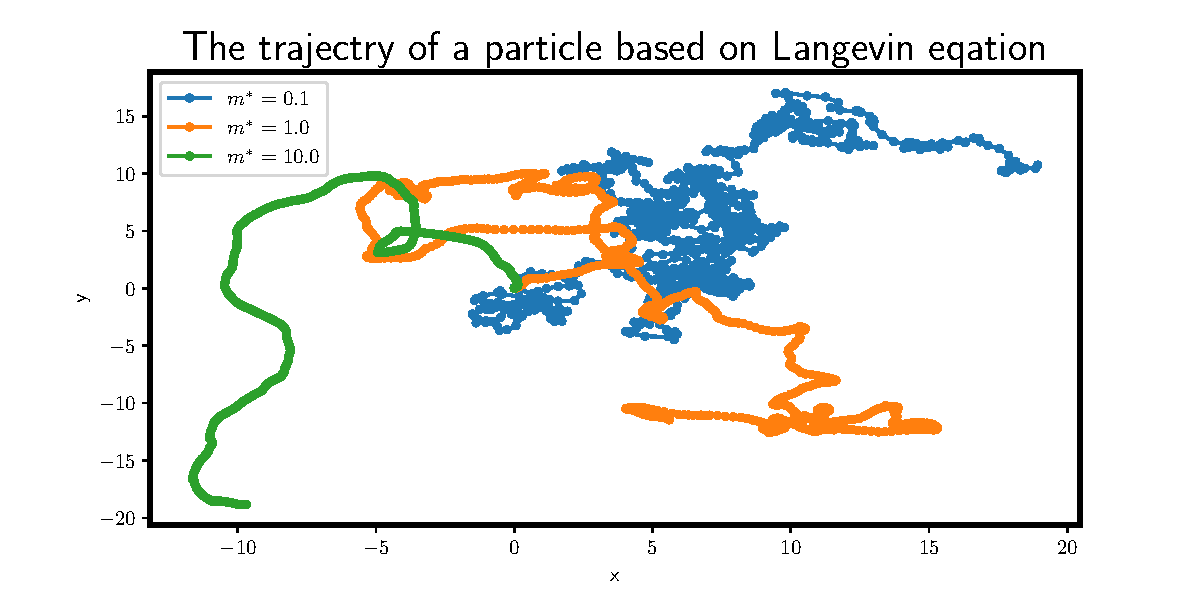
\includegraphics[scale=0.4]{problem_1/1-4/problem1-4.pdf}
    \caption{Langevin熱浴中における1粒子のブラウン運動}
\end{figure}
この図より, 慣性質量が大きくなるほど, 時間あたりの粒子の変位は小さくなっていることが分かる.


% (5)
\subsection{}
\noindent
10000個の粒子について(4)と同じシミュレーションを行い, 時間変化による平均二乗変位を求めた.
プログラムの実行手順としては, まずproblem1-5 langevin.cppですべての粒子座標の時間発展を出力し, 
それをproblem1-5 analyze.cppで解析した.
それらのデータをもとにproblem1.ipynbを用いてプロットした.
また(3)で求めた式(1.10)を理論式として同じグラフにプロットした.
これらの結果を図2に示す.

\begin{figure}[H]
    \centering
    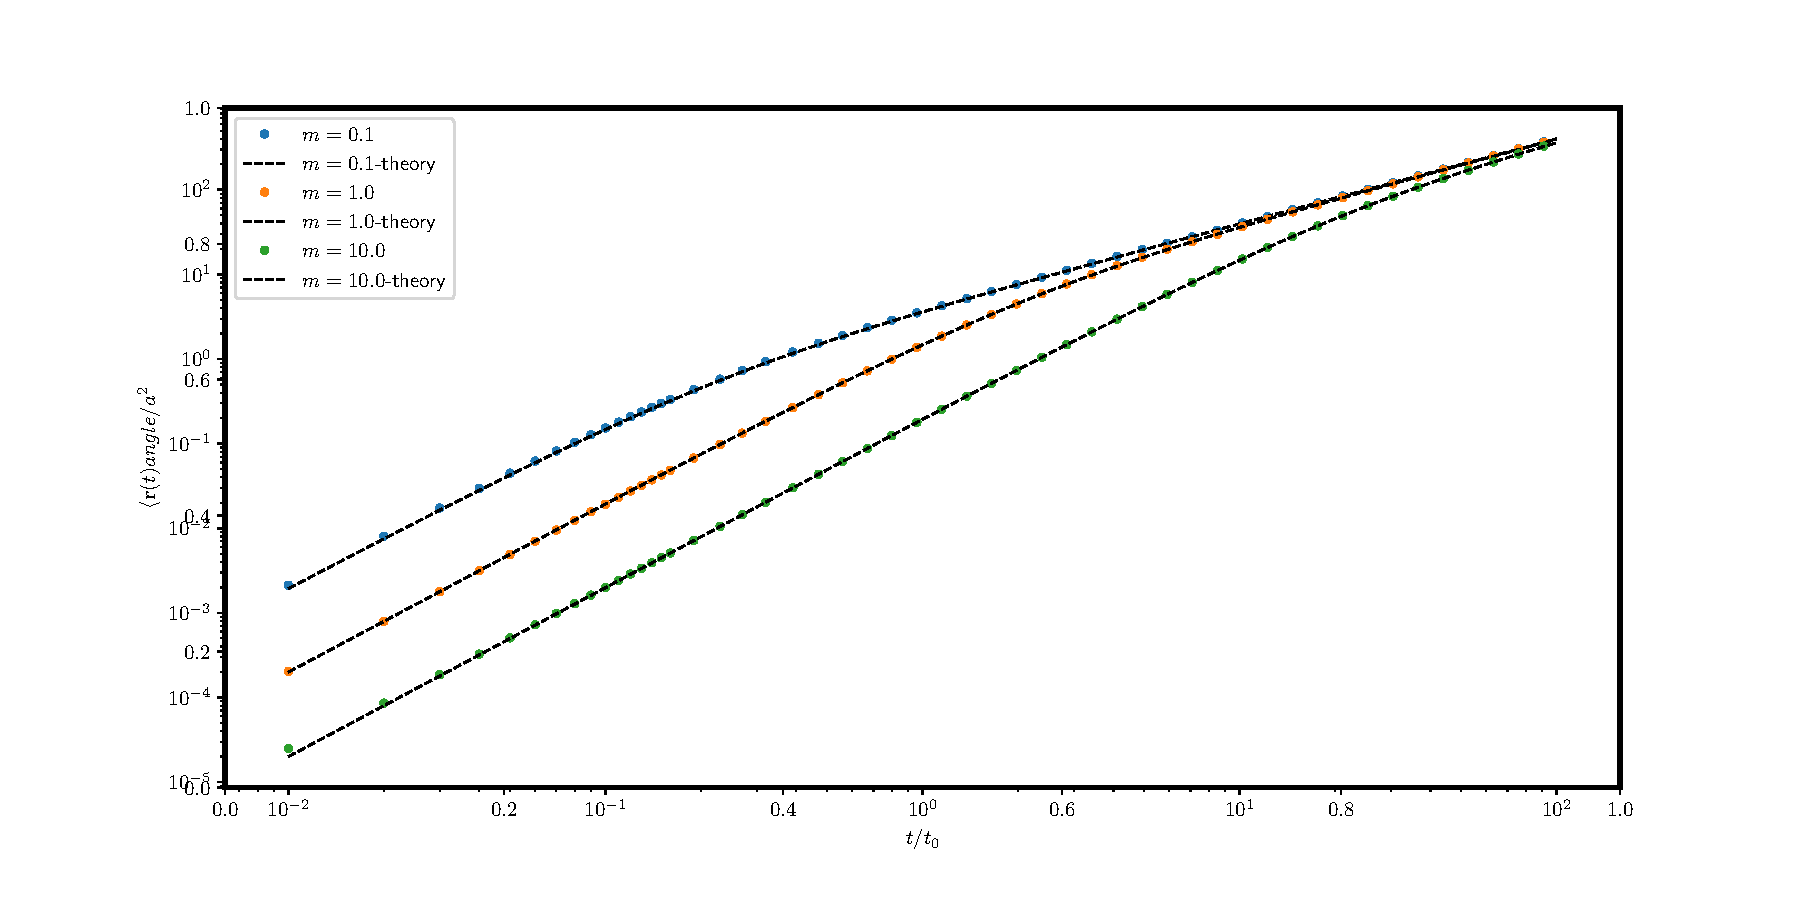
\includegraphics[scale=0.4]{problem_1/1-5/problem1-5.pdf}
    \caption{Langevin熱浴中における粒子の平均二乗変位}
\end{figure}
これを見ると, シミュレーションで求めた数値と理論式はよく一致している.

\noindent
この図より, 慣性質量が増加すると(4)で考察したように時間当たりの粒子の変位が
小さくなることから, 弾性領域においては平均二乗変位が減少する. 
拡散領域においては時間あたりの変位が小さくなり, 時間経過とともに収束していく.


\newpage

% 問題2
\section{}
% (1)
\subsection{}
\noindent
与えられた $U(r)$ に $r=r_{cut}$ を代入すると

\begin{align*}
    U(r_{cut}) &= U_0(r_{cut}) - u_0(r_{cut}) - U_0'(r_{cut}) (r_{cut} - r_{cut}) \\
    &= 0 \tag{2.1}
\end{align*}
また

\begin{equation}
    U'(r) = U_0''(r - r_{cut}) \tag{2.2}
\end{equation}
より

\begin{align*}
    U'(r_{cut}) &= U_0''(r_{cut} - r_{cut}) \\
    &= 0 \tag{2.3}
\end{align*}

% (2)
\subsection{}
\noindent
与えられた $U_0(r)$ について

\begin{align*}
    U_0'(r) &= 4 \epsilon \qty{-\frac{12a^{12}}{r^{13}} + \frac{6a^6}{r^7}} \\ 
    &= 24 \epsilon \qty{-\frac{2a^{12}}{r^{13}} + \frac{a^6}{r^7}} \tag{2.4}
\end{align*}
より, 今回用いる平滑化ポテンシャルは

\begin{equation}
    U(r) = 4 \epsilon \qty{\qty(\frac{a}{r})^{12} - \qty(\frac{a}{r})^6}
    - 24 \epsilon \qty{-\frac{2a^{12}}{r_{cut}^{13}} + \frac{a^6}{r_{cut}^7}} r
    + C \tag{2.5}
\end{equation}
ここで $C$ はrによらない定数. 
式(2.5)をrについて微分すると
\begin{equation}
    U'(r) = 24 \epsilon \qty{-\frac{2a^{12}}{r^{13}} + \frac{a^6}{r^7}}
    - 24 \epsilon \qty{-\frac{2a^{12}}{r_{cut}^{13}} + \frac{a^6}{r_{cut}^7}} 
    \tag{2.6}
\end{equation}
これを用いてシミュレーションを行う.

\noindent
与えられた条件でシミュレーションを行った後の1000個の2次元円盤粒子の配置を図3に示す.
なお, 粒子の初期位置は正方格子とした.
シミュレーションの実行手順としては, まずデータをproblem2-2.cppで出力し, 
その後problem2.ipynbを用いてプロットした.

\begin{figure}[H]
    \centering
    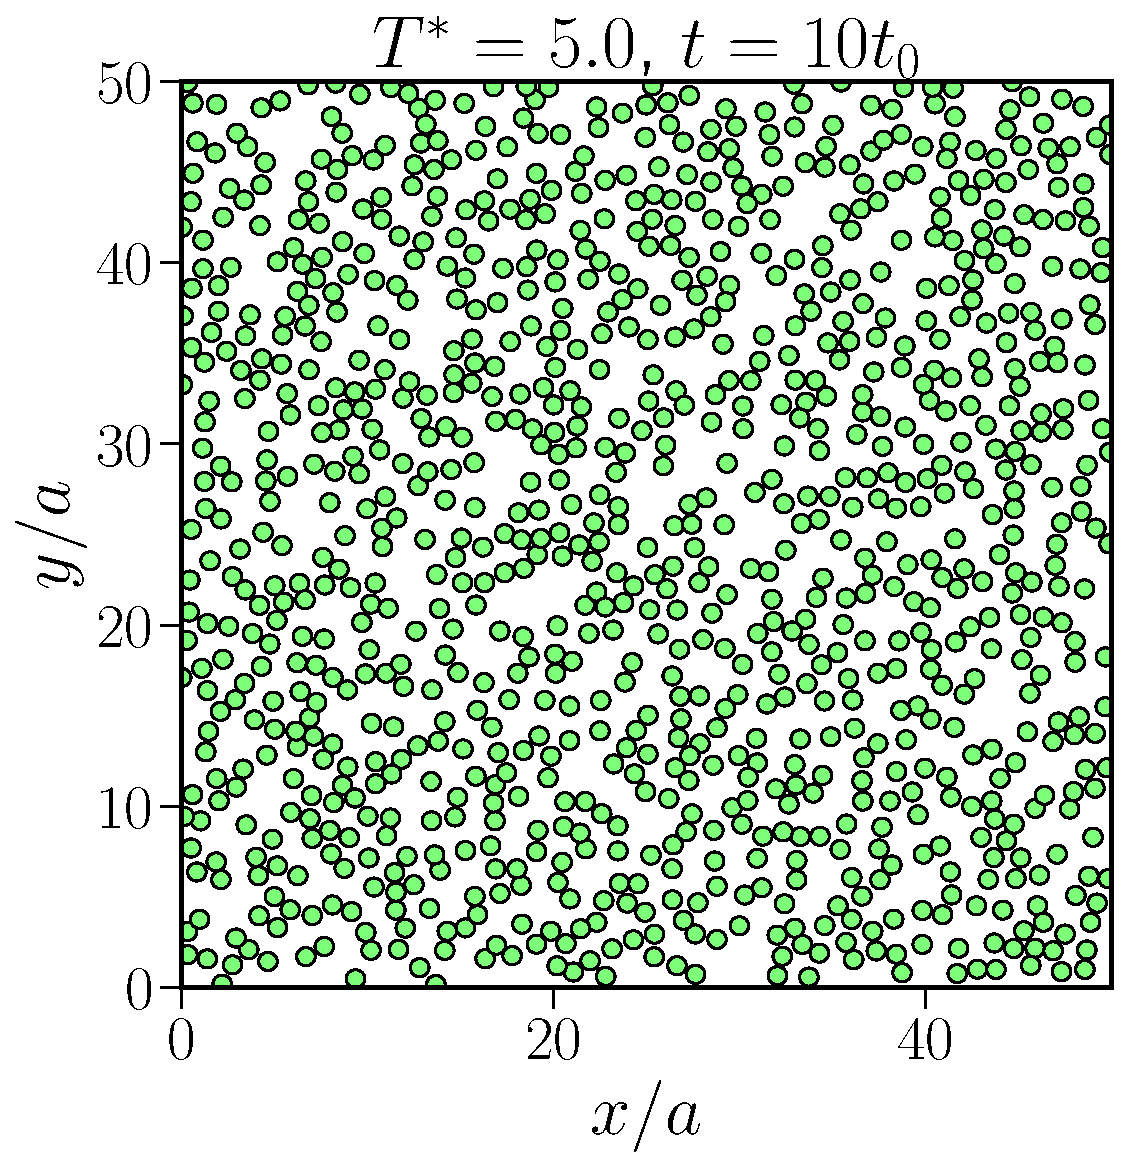
\includegraphics[scale=0.6]{problem_2/2-2/problem2-2.pdf}
    \caption{$T^*=5.0$ , 時間 $10t_0$ のシミュレーション後の2次元円盤粒子配置}
\end{figure}

% (3)
\subsection{}
\noindent
与えられた条件でシミュレーションを行った後の1000個の2次元円盤粒子の配置を図4に示す.
なお, 粒子の初期位置,速度は(2)の配置とした.
シミュレーションの実行手順としては, まずデータをproblem2-3.cppで出力し, 
その後problem2.ipynbを用いてプロットした.

\begin{figure}[H]
    \centering
    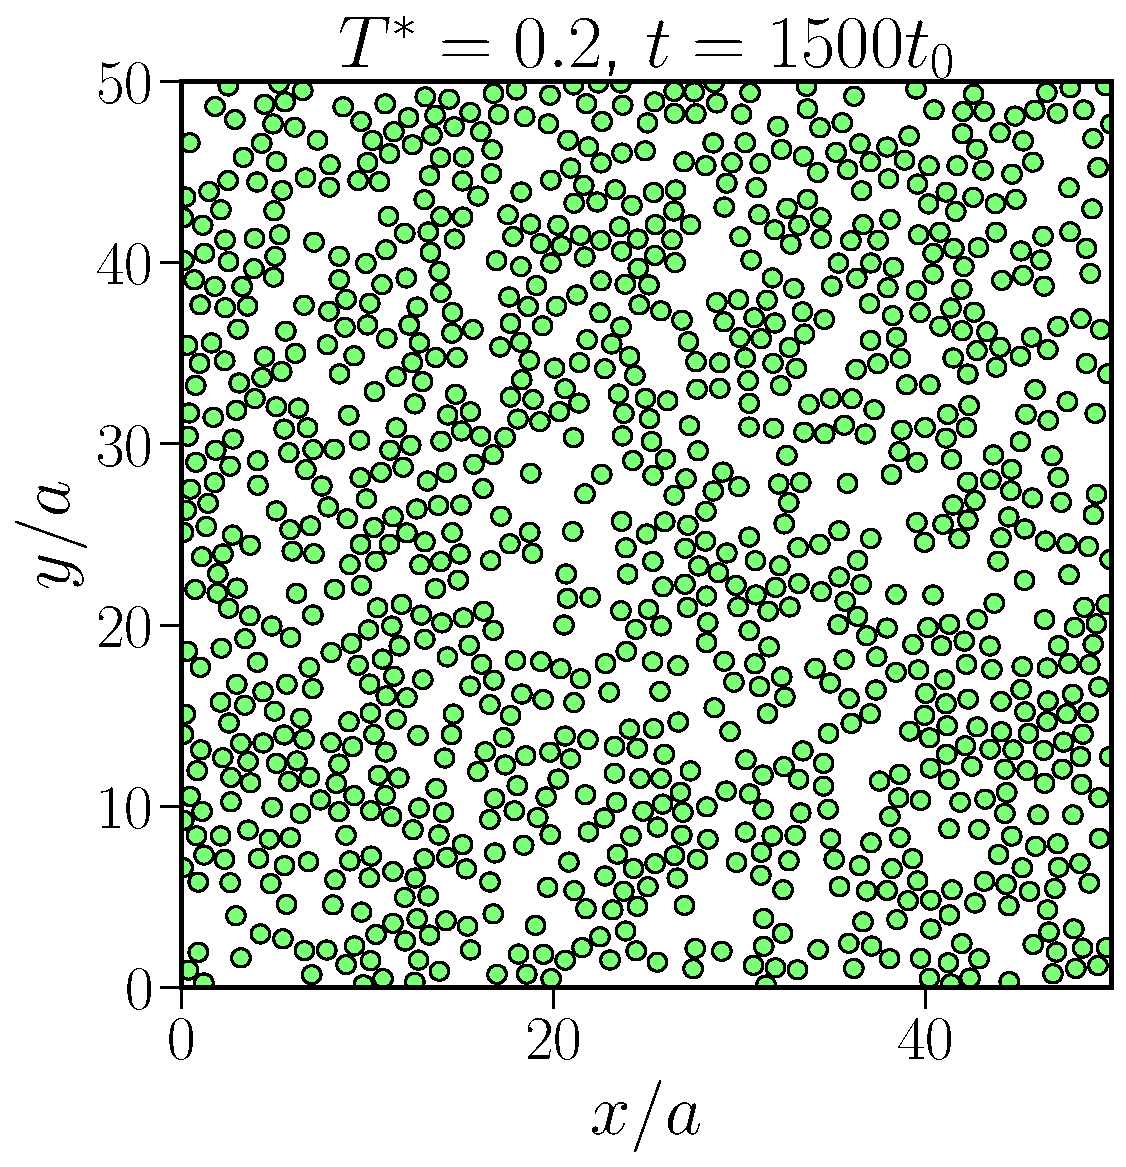
\includegraphics[scale=0.6]{problem_2/2-3/problem2-3.pdf}
    \caption{$T^*=0.2$ , 時間 $1500t_0$ のシミュレーション後の2次元円盤粒子配置}
\end{figure}


% % (4)
% \subsection{}
% \noindent
% 与えられた条件でシミュレーションを行った後の1000個の2次元円盤粒子の配置を図4に示す.
% なお, 粒子の初期位置,速度は(3)の配置とした.
% シミュレーションの実行手順としては, まずデータをproblem2-4.cppで出力し, 
% その後problem2.ipynbを用いてプロットした.

% (5)
\subsection{}
\noindent
与えられたMaxwell-Boltzmann分布に $T^*=\frac{k_B}{T}$ を代入すると

\begin{equation}
    f(v_x) = \sqrt{\frac{m}{2\pi \epsilon T^*}}e^{-\frac{mv_x^2}{2\epsilon T^*}} \tag{2.7}
\end{equation}
$f(v_x)$ は速さの逆数を持っていることと $v=\frac{a}{t_0}\tilde{v}$ より
$f(v_x)=\frac{t_0}{a} \tilde{f}(\tilde{v_x})$ . 
よって $t_0=\sqrt{\frac{ma^2}{\epsilon}}$ より

\begin{align*}
    \tilde{f}(\tilde{v_x}) &= \frac{a}{t_0}\sqrt{\frac{m}{2\pi \epsilon T^*}}e^{-\frac{ma^2\tilde{v_x}^2}{2t_0^2\epsilon T^*}} \\
    &= \sqrt{\frac{1}{2\pi T^*}}e^{-\frac{\tilde{v_x}^2}{2T^*}} \tag{2.8}
\end{align*}
となり, 題意に適する.

% % (6)
% \subsection{}
% \noindent

\newpage
\noindent
※添付ファイル \\
・langevin.py \\
・problem1-5 langevin.cpp \\
・problem1-5 analyze.cpp \\
・ploblem2-2.cpp \\
・problem2-3.cpp  \\
・ploblem1.ipynb \\
・ploblem2.ipynb

\end{document}